\subsection{Encapsulamento}

Até então, quando foi realizada a criação de propriedades para a
classe, elas foram definidas com a visibilidade: privada, do inglês,
\textit{private}. Sendo que, sempre que define-se propriedades e métodos em
uma classe deve-se informar qual a  sua visibilidade. Por conseguinte, existem
três visibilidades, são elas: privada, protegida e pública. Segundo
\citeonline{javaComoProgramar}, os conceitos de visibilidade também são
chamados de modificadores de acesso.

A visibilidade privada, do inglês \textit{private}, permite acesso somente
dentro do escopo da classe que definiu a propriedade ou método. Enquanto que, a
visibilidade protegida, do inglês \textit{protected}, permite que todas as
classes  que herdam propriedades ou métodos tenham acesso dentro do escopo da classe filha.
Em contrapartida, a visibilidade pública, do inglês \textit{public}, permite que
qualquer objeto que tenha instanciado um objeto da classe que definiu uma propriedade ou
método, possa invocá-lo no caso do método, ou modificar o seu estado no caso de
uma propriedade \cite{learningJava}.

Por questões de segurança da aplicação é interessante fornecer
interfaces para manipulação dos estados de um objeto. Por conta disto,  sempre
que define-se uma propriedade em uma classe, utiliza-se a visibilidade
privada, caso essa classe não implemente conceitos de herança posteriormente,
ou então, usa-se a visibilidade protegida a fim de permitir que as classes
especialistas  herdem as suas definições. E, é justamente este o conceito de
encapsulamento, realizar o ocultamento dos dados ou informações \cite{javaComoProgramar}.

Mas para que um cliente de um objeto – todos os objetos que estão fora do
escopo da classe - possa modificar os estados das propriedades, são criados
métodos especialistas conhecidos como: métodos \textit{getters} e \textit{setters}.

\subsubsection{Métodos getters e setters}

São métodos responsáveis por modificar e recuperar os estados de uma variável
membro de uma classe, permitindo que esta função membro esteja exposta a todo o
escopo da aplicação.

Na sequência, apresenta-se em detalhes as linhas de código exibidas na Figura
\ref{fig:methodGettersAndSetters}:

\begin{alineas}
    \item linha 3: vê-se a declaração da classe \textit{Carro};
    \item linha 5: define-se a propriedade \textbf{\$cor};
    \item linha 7: cria-se um método responsável por recuperar o valor da
    propridade \textbf{\$cor} que recebe o nome de \textit{getCor};
    \item linha 12: implementa-se um método responsável por modificar o estado
    da propriedade cor, sendo que, o método é nomeado como \textit{setCor}.
\end{alineas}

Na Figura \ref{fig:methodGettersAndSetters}, é apresentado um exemplo
de implementação do padrão de métodos \textit{getters and setters} na
linguagem \acs{PHP}:

\begin{figure}[h!tb]
	\caption{Métodos getters e setters na linguagem PHP}
	\label{fig:methodGettersAndSetters}

	\centering
	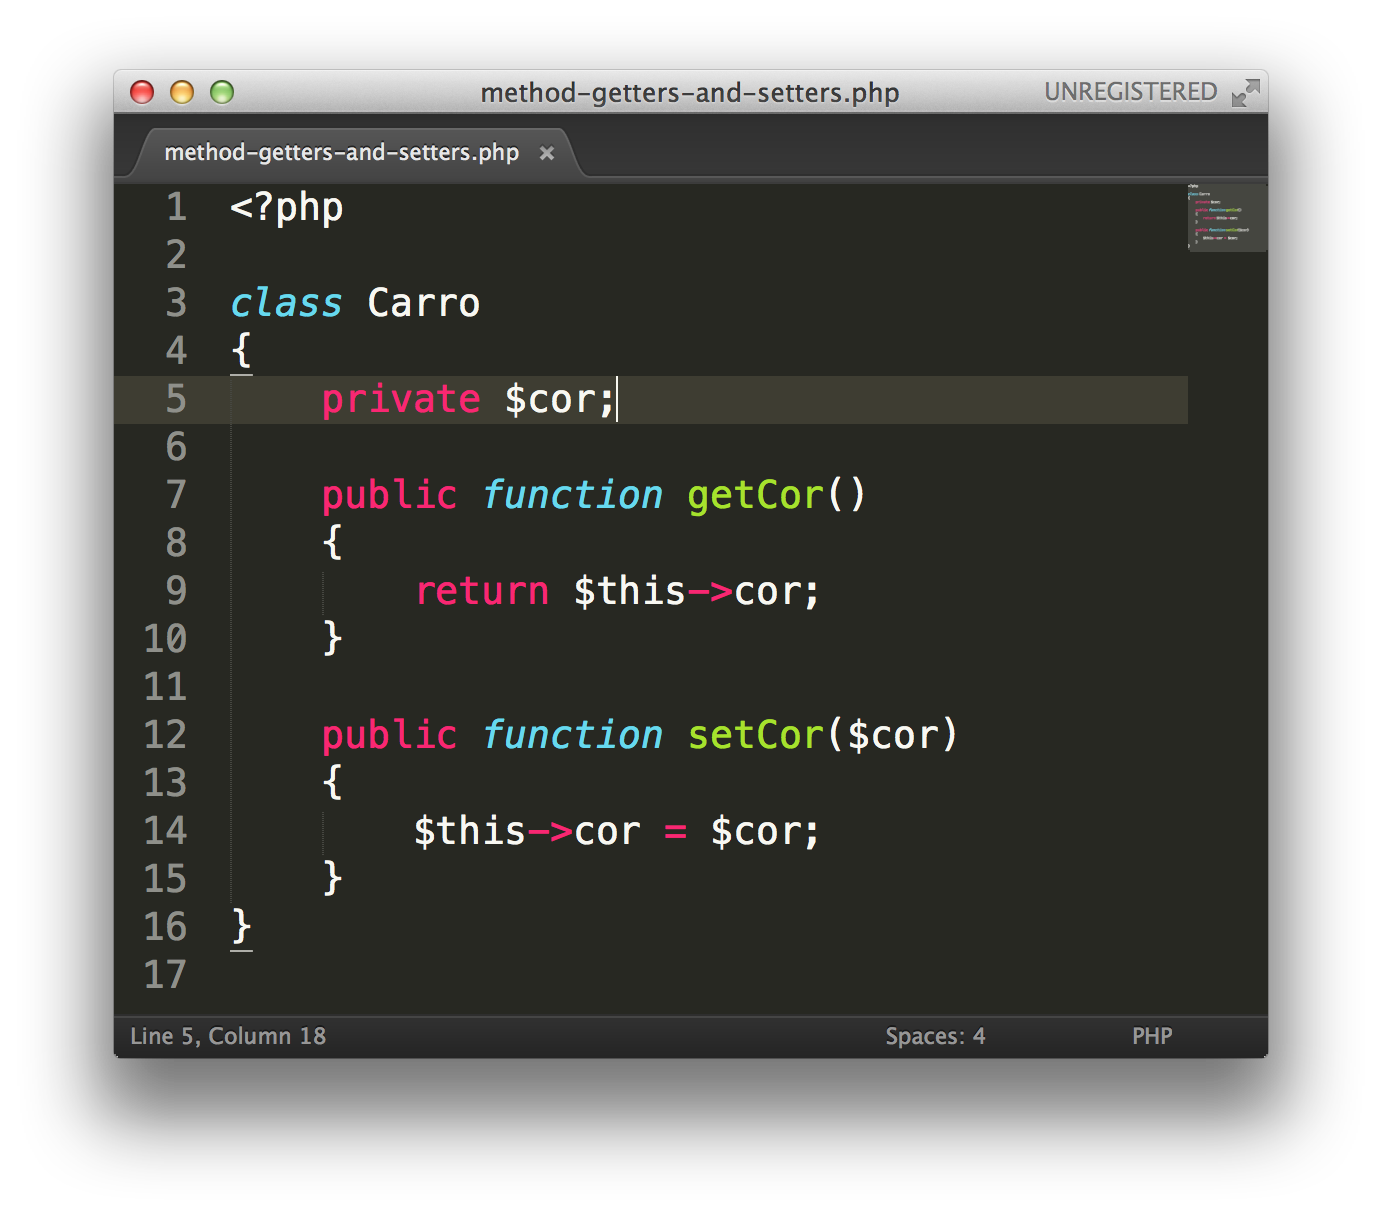
\includegraphics[width=0.75\textwidth]{images/method-getters-and-setters.png}

	\centering
	\footnotesize Fonte: \fonteOAutor
\end{figure}

\FloatBarrier 	% Este comando impede que as imagens
				% flutuem a partir deste ponto no seu documento

No caso do método configurar, do inglês \textit{set}, ele permite que os
clientes de um objeto configurem novos valores para uma propriedade, realizando
antecipadamente uma ação para validar a entrada de dados.

Em contrapartida, existe o método obter, do inglês \textit{get}, que recupera o
valor de uma propriedade, sendo que, este método poderia realizar, por exemplo,
uma formatação adequada de uma propriedade.

Sendo que, o nome desses métodos (por conta de uma convenção de atribuição de
nomes) recebe o prefixo \textit{set} ou \textit{get} seguido do nome da
propriedade, tendo esta a sua primeira letra em caixa alta \cite{javaComoProgramar}.

A seguir será apresentada uma forma elegante de tratar erros em uma aplicação
orientada a objetos através de Exceções.